% ****** Start of file apssamp.tex ******
%
%   This file is part of the APS files in the REVTeX 4.1 distribution.
%   Version 4.1r of REVTeX, August 2010
%
%   Copyright (c) 2009, 2010 The American Physical Society.
%
%   See the REVTeX 4 README file for restrictions and more information.
%
% TeX'ing this file requires that you have AMS-LaTeX 2.0 installed
% as well as the rest of the prerequisites for REVTeX 4.1
%
% See the REVTeX 4 README file
% It also requires running BibTeX. The commands are as follows:
%
%  1)  latex apssamp.tex
%  2)  bibtex apssamp
%  3)  latex apssamp.tex
%  4)  latex apssamp.tex
%
\documentclass[%
reprint,
%superscriptaddress,
%groupedaddress,
%unsortedaddress,
%runinaddress,
%frontmatterverbose, 
%preprint,
%showpacs,preprintnumbers,
%nofootinbib,
%nobibnotes,
%bibnotes,
amsmath,amssymb,
aps,
%pra,
%prb,
%rmp,
%prstab,
%prstper,
%floatfix,
]{revtex4-1}

\usepackage{graphicx}% Include figure files
\usepackage{dcolumn}% Align table columns on decimal point
\usepackage{bm}% bold math
\usepackage{hyperref}% add hypertext capabilities
%\usepackage[mathlines]{lineno}% Enable numbering of text and display math
%\linenumbers\relax % Commence numbering lines

%\usepackage[showframe,%Uncomment any one of the following lines to test 
%%scale=0.7, marginratio={1:1, 2:3}, ignoreall,% default settings
%%text={7in,10in},centering,
%%margin=1.5in,
%%total={6.5in,8.75in}, top=1.2in, left=0.9in, includefoot,
%%height=10in,a5paper,hmargin={3cm,0.8in},
%]{geometry}

\begin{document}
	
	\preprint{APS/123-QED}
	
	\title{Medevial Siege Weapons}% Force line breaks with \\
	
	
	\author{Bikun Li}
	
	\author{Hong Yao}%
	
	\affiliation{%
		Department of Physics, Virginia Tech, Blacksburg, VA 24060, USA 
	}%
	
	
	
	\date{\today}% It is always \today, today,
	%  but any date may be explicitly specified
	
	
	\maketitle
	
	%\tableofcontents
	
	\section{\label{sec:level1}Introduction}
	
	Medieval siege weapons convert some form of potential energy into the kinetic energy of the
	projectile. Before the arrival of gun powder and canons on the battlefield they were the artillery
	of their time, the 12th – 15th century.
	
	The specific weapon we will be studying is called a trebuchet, and here the potential energy of
	a counterweight is converted into the kinetic energy of the projectile.
	\begin{figure}
		\centering
		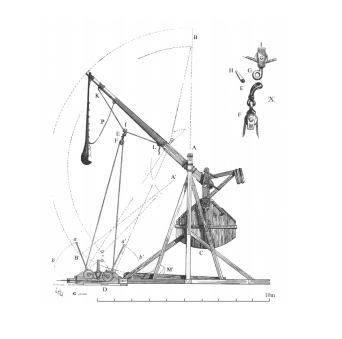
\includegraphics[scale=0.8]{Intro.png}
		\caption{Trebuchet}
		%\label{fig:my_label}
	\end{figure}
	\linebreak
	\section{\label{sec:level2} Energy Efficiency and Range Efficiency of a Trebuchet}
	In this section, we calculate the general energy efficiency and range efficiency of a trebuchet. We also show the relation between these two efficiencies.
	\subsection{Energy Efficiency}
	The definition of the energy efficiency $\epsilon_E$ is the  fraction of available potential energy is converted
	to the kinetic energy of the projectile
	\begin{equation}
	\epsilon_E=\frac{m_2v_0^2}{2m_1gh},
	\label{EnergyEff}
	\end{equation}
	where $v_0$ is the initial velocity of the projectile and $h$ is the height the counterweight $m_1$ fell. 
	\subsection{Range Efficiency}
	The definition of the range efficiency is  fraction of range of the
	theoretical maximum range can be achieved
	\begin{equation}
	\epsilon_R=\frac{R}{R_{\mathrm{max}}}.
	\end{equation}
	For a projectile showed in Fig.(2), 
	\begin{figure}
		\centering
		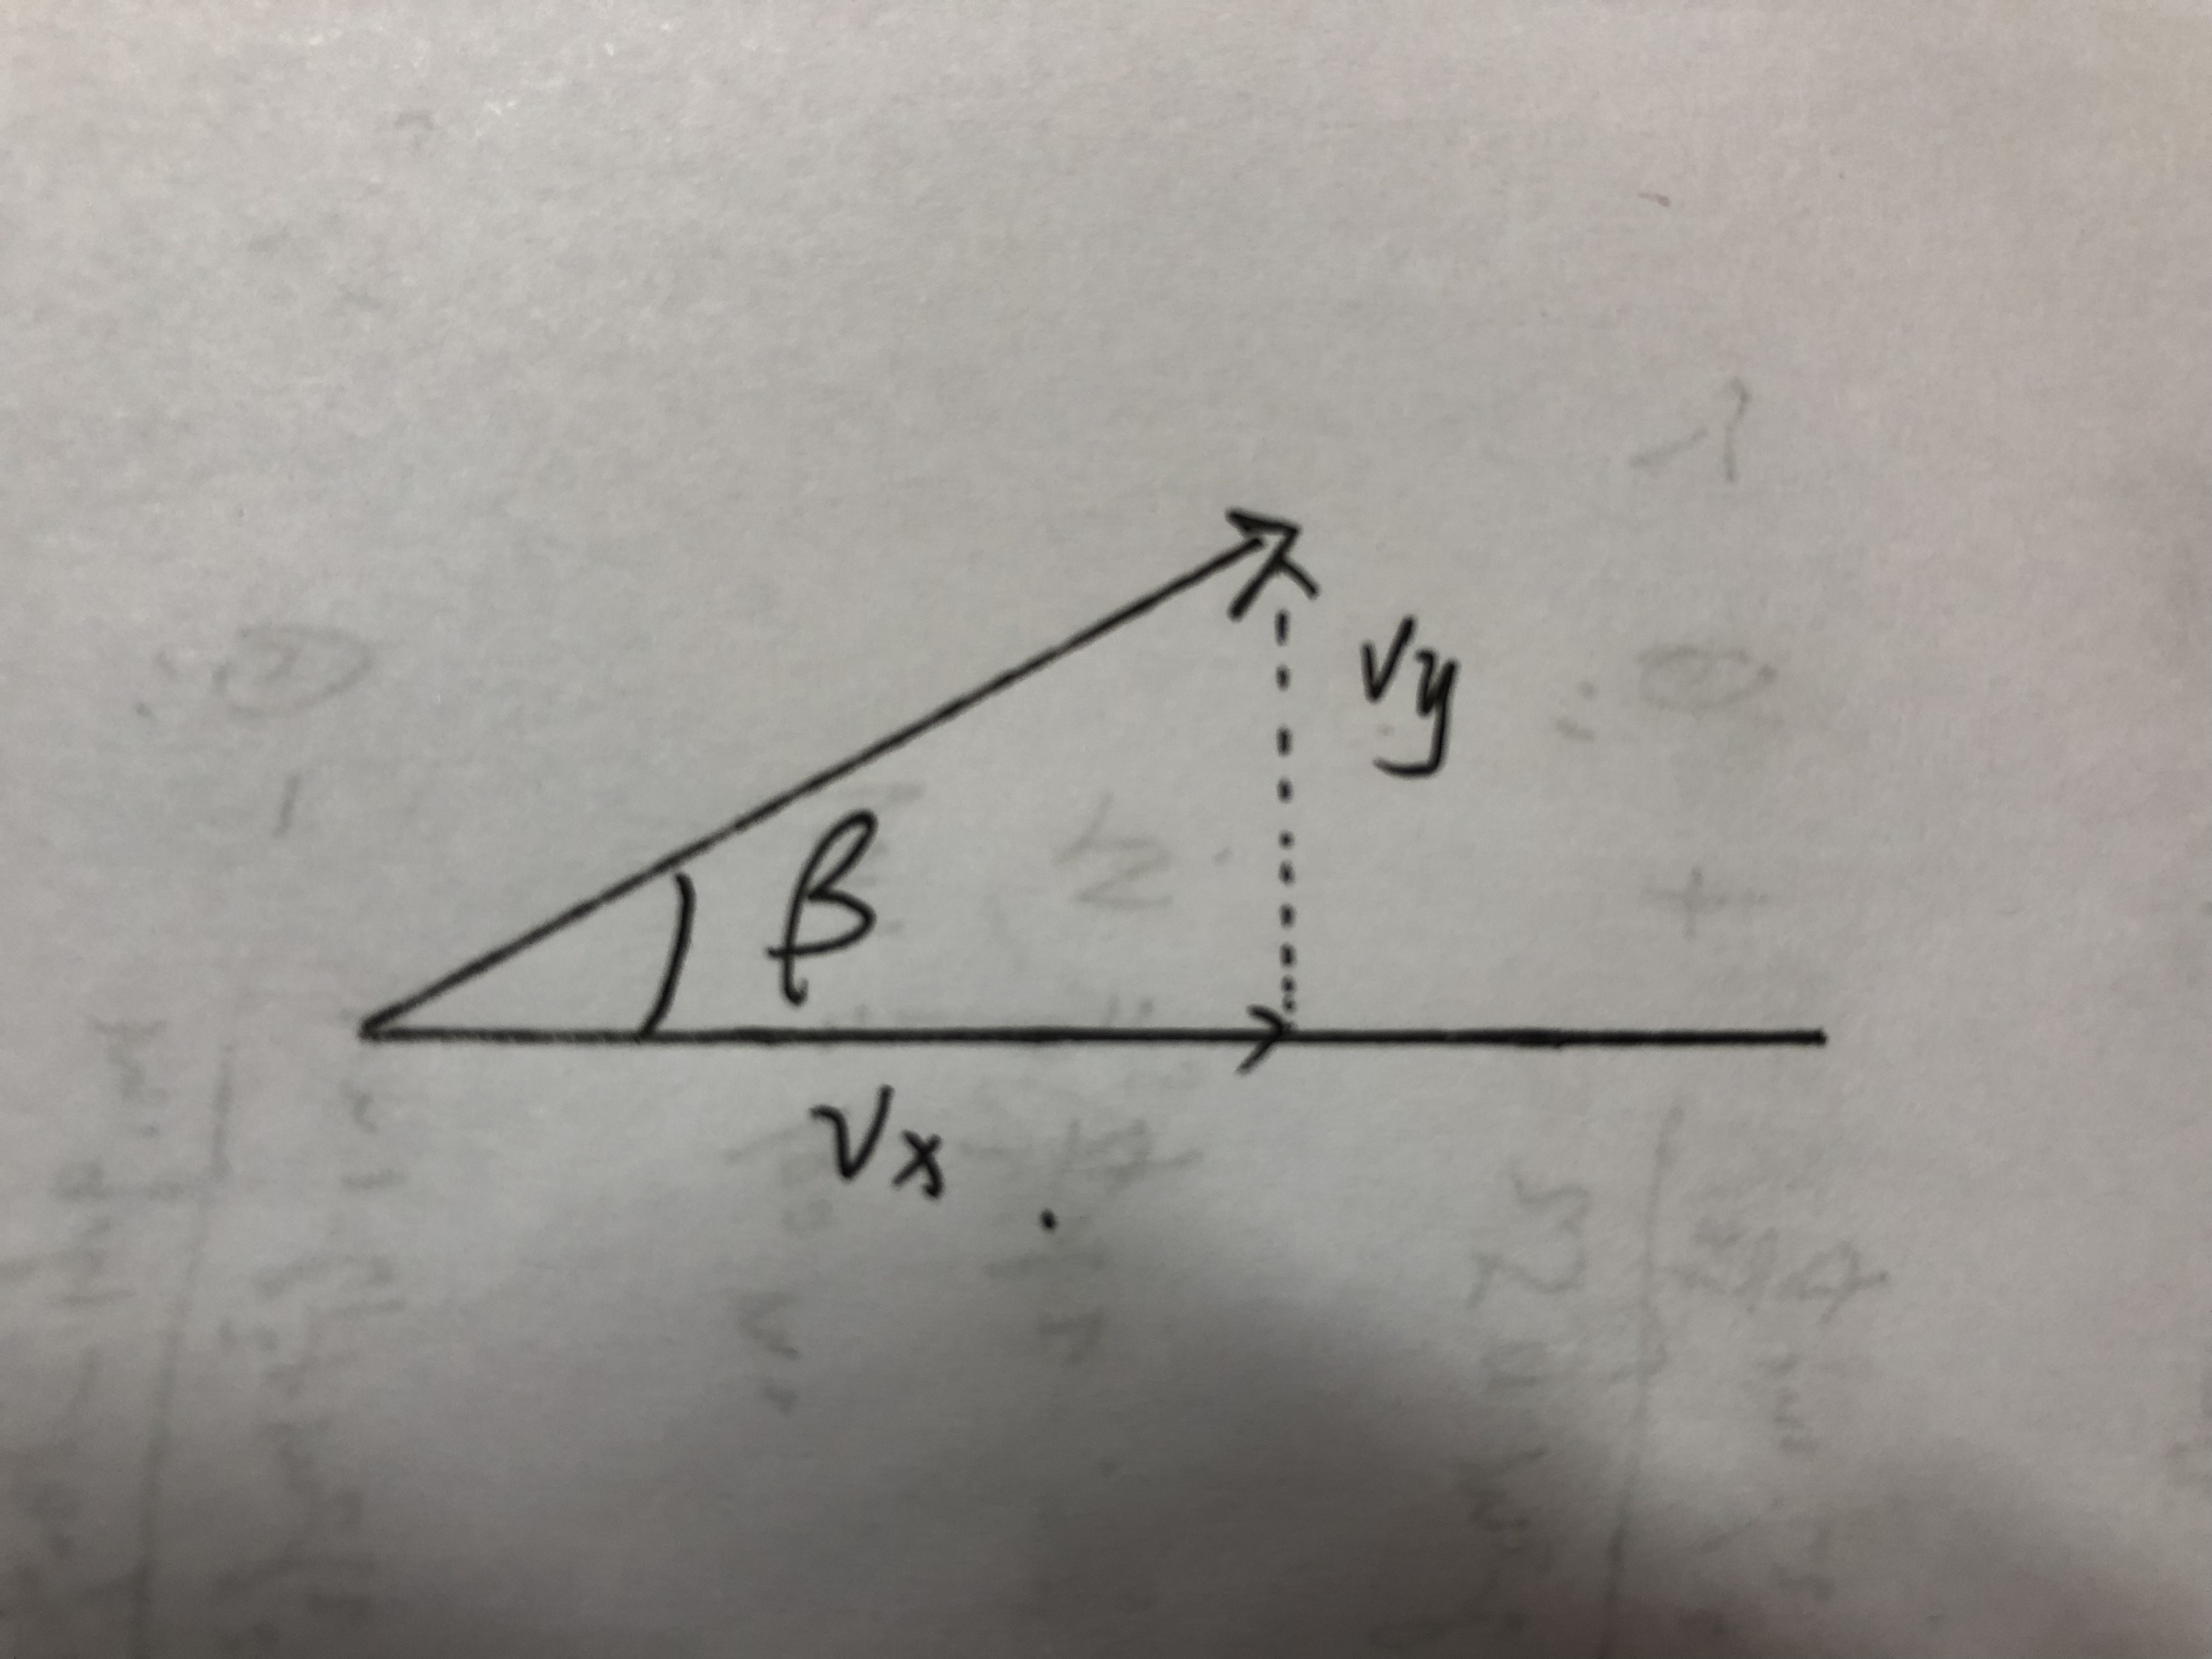
\includegraphics[scale=0.05]{ProjectedAngle.jpg}
		\caption{Projected Angle $\beta$}
		%\label{fig:my_label}
	\end{figure}
	we know the range is 
	\begin{equation}
	R=\frac{v_0^2}{g}\sin{2\beta},
	\label{rangeofprojection}
	\end{equation}
	where $g=9.8m/s^2$ and $\beta$ is the projected angle showed in Fig.(2).
	
	For the theoretical maximum range, we have the theoretical maximum initial projected velocity, which means we transfer ALL the potential energy of the counterweight to the kinetic energy of the projectile
	\begin{equation}
	\frac{1}{2}m_2v_{\mathrm{max}}^2=m_1gh.
	\end{equation}
	Thus, we have $R_{\mathrm{max}}$
	\begin{equation}
	R_{\mathrm{max}}=\frac{v_{\mathrm{max}}^2\sin(2\pi/4)}{g}=2\frac{m_1}{m_2}h
	\end{equation}
	Thus, we have the range efficiency
	\begin{equation}
	\epsilon_R=\frac{\frac{v_0^2}{g}\sin{2\beta}}{2\frac{m_1}{m_2}h} = \frac{m_2 v_0^2}{2m_1gh}\sin 2\beta\;.
	\label{rangeEff}
	\end{equation}
	\subsection{Relation Between Two Efficiencies}
	From the Eq.(\ref{EnergyEff}) and Eq.(\ref{rangeEff}), it is easy to find out the relation between range efficiency $\epsilon_R$ and energy efficiency $\epsilon_E$
	\begin{equation}
	\epsilon_R=\epsilon_E\sin{2\beta}
	\end{equation}
	\newline\newline
	\section{The See-saw Trebuchet}
	In this section, we study the mechanism of See-saw trebuchet. We give the equation of motion of the system before the projectile and give the numerical solution of it. We also find out the release angle $\theta_R$ which maximize the range and find out the energy and range efficiency at that release angle.
	\begin{figure}
		\centering
		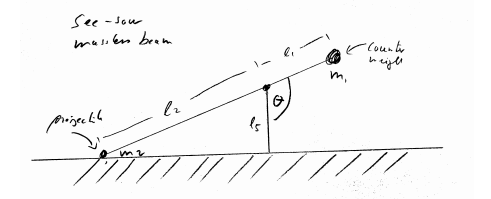
\includegraphics[scale=0.6]{Seesawmodel.png}
		\caption{See-saw Trebuchet}
		%\label{fig:my_label}
	\end{figure}
	\subsection{The Motion before Released}
	For the motion before released, we have the Lagrangian
	\begin{equation}
	L=\frac{1}{2}m_1l_1^2\dot{\theta}^2+\frac{1}{2}m_2l_2^2\dot{\theta}^2+(m_1gl_1-m_2gl_2)\cos{\theta}
	\end{equation}
	Thus, we have the Euler-Lagrange equation
	\begin{equation}
	\ddot{\theta}+\frac{m_1gl_1-m_2gl_2}{m_1l_1^2+m_2l_2^2}\sin{\theta}=0
	\end{equation}
	Take $m_2 = 0.5$ kg, $m_1 = 50$kg, $l_1 = 0.3$m, $l_2 = 1.2$m and $\theta(t=0) = 135^\circ$ and all velocities
	as zero. We finally have
	\begin{equation}
	\ddot{\theta}+27.034(s^{-1})\sin\theta=0.
	\end{equation}
	\begin{figure}
		\centering
		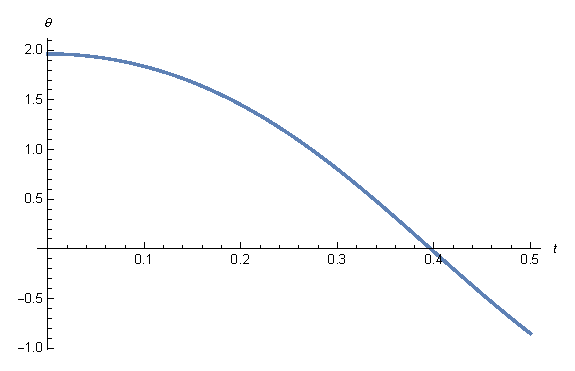
\includegraphics[scale=0.8]{See-Saw.eps}
		\caption{The Motion of the System before Released}
		%\label{fig:my_label}
	\end{figure}
	By numerically solving this equation, the results are showing in Fig.(4).
	\subsection{Release Angle for Maximum Range}
	We set $\alpha=\pi/2-\theta_R$, which is showed in Fig.(5).
	The motion after released is a projectile. From Eq.(\ref{rangeofprojection}), we know
	\begin{equation}
	R=\frac{v_0^2}{g}\sin(2\beta)
	\end{equation}
	where $\beta=\pi/2-\alpha$.
	\begin{figure}
		\centering
		\includegraphics[scale=0.05]{anglealpha.jpg}
		\caption{Relation between $\theta$ and $\alpha$}
		%\label{fig:my_label}
	\end{figure}
	
	Then, we have to find out $v_0$. From the energy conservation of the first part of the motion, we have
	\begin{equation}
	(m_1gl_1-m_2gl_2)(\sin{\pi/4}+\sin{\alpha})
	=\left(\frac{1}{2}m_1l_1^2+\frac{1}{2}m_2l_2^2\right)\omega^2,
	\end{equation}
	where $v_0=\omega l_2$.
	Thus,
	\begin{equation}
	v_0^2=l_2^2\frac{(m_1gl_1-m_2gl_2)(\sqrt{2}+2\sin{\alpha})}{m_1l_1^2+m_2l_2^2}.
	\end{equation}
	We can find out the function of the range about angle $\alpha$
	\begin{equation}
	R=l_2^2\frac{(m_1l_1-m_2l_2)(\sqrt{2}+2\sin{\alpha})}{m_1l_1^2+m_2l_2^2}\cdot\sin{2\alpha}.
	\end{equation}
	The relation between the range and angle $\alpha$ is showed in Fig.(6).
	\begin{figure}[h]
		\centering
		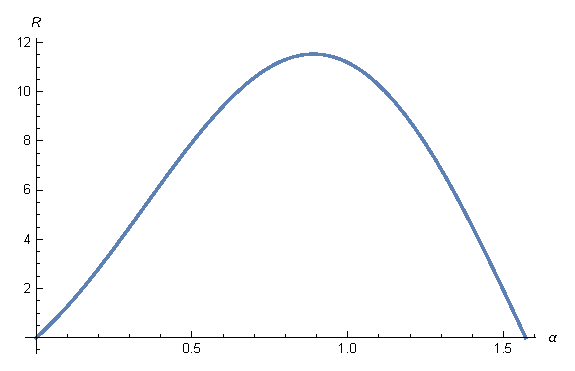
\includegraphics[scale=0.8]{See-SawRangevsAlpha.eps}
		\caption{Relation between Range and $\alpha$.}
		\label{fig:my_label1}
	\end{figure}
	With the relation $\alpha=\pi/2-\theta_R$, we have the relation between range and $\theta$
	\begin{equation}
	R=l_2^2\frac{(m_1l_1-m_2l_2)(\sqrt{2}+2\cos{\theta})}{m_1l_1^2+m_2l_2^2}\cdot\sin{2\theta}.
	\end{equation}
	The relation is showed in Fig.(7).
	\begin{figure}[h]
		\centering
		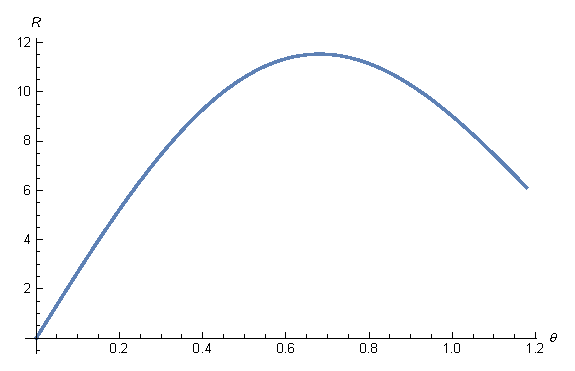
\includegraphics[scale=0.8]{See-SawRangevsTheta.eps}
		\caption{Relation between Range and $\theta$.}
		%different range between label1,2?
		\label{fig:my_label2}
	\end{figure}
	With
	\begin{equation}
	\frac{dR}{d\alpha}=0
	\end{equation}
	or
	\begin{equation}
	\frac{dR}{d\theta}=0
	\end{equation}
	we can find the extremum of the range. And we have 
	\begin{equation}
	\begin{aligned}
	\alpha_R&=0.8898\approx 0.283\pi
	\\
	\theta_R&=0.6810\approx 0.216\pi
	\end{aligned}.
	\end{equation}
	\subsection{The efficiencies of See-saw Trebuchet}
	With the released angle, we can find out the potential energy of counterweight and the kinetic energy of the projector.
	\begin{equation}
	\begin{aligned}
	E_k&=\frac{1}{2}m_2l_2^2\omega^2
	\\&=\frac{1}{2}m_2l_2^2\frac{m_1gl_1-m_2gl_2)(\sqrt{2}+2\sin{\alpha_R})}{m_1l_1^2+m_2l_2^2}
	\\&=28.8856(J)
	\end{aligned}
	\end{equation}
	and
	\begin{equation}
	E_p=m_1gh=m_1gl_1(\sqrt{2}+2\sin\alpha_R)=226.5356(J)
	\end{equation}
	Finally, we have
	\begin{equation}
	\epsilon_E=\frac{E_k}{E_p}=0.1324.
	\end{equation}
	
	With the released angle, we can calculate the range
	\begin{equation}
	\begin{aligned}
	R&=l_2^2\frac{(m_1l_1-m_2l_2)(\sqrt{2}+2\sin{\alpha_R})}{m_1l_1^2+m_2l_2^2}\cdot\sin{2\alpha_R}\\&=11.5344(m).
	\end{aligned}
	\end{equation}
	We can also calculate the optimized range
	\begin{equation}
	R_{\mathrm{opt}}=\frac{2m_1}{m_2}h=\frac{m_1}{m_2}l_1(\sqrt{2}+2\sin\alpha)=89.0432(m).
	\end{equation}
	Thus, the range efficiency is 
	\begin{equation}
	\epsilon_R=\frac{R_{\mathrm{opt}}}{R_{\mathrm{max}}}=0.1295.
	\end{equation}
	We can check the relation in Section 1.
	\begin{equation}
	\epsilon_E\sin{2\alpha_R}=0.1324\times0.978=0.1295=\epsilon_R.
	\end{equation}
	\newline\newline
	\newpage
	\section{See-saw Trebuchet with Hinged Counterweight}
	In this section, we study the mechanism of See-saw trebuchet with hinged counterweight. We give the equation of motion of the system before the projectile and give the numerical solution of it. We also find out the release angle $\theta_R$ which maximize the range and find out the energy and range efficiency at that release angle.
	\begin{figure}[h]
		\centering
		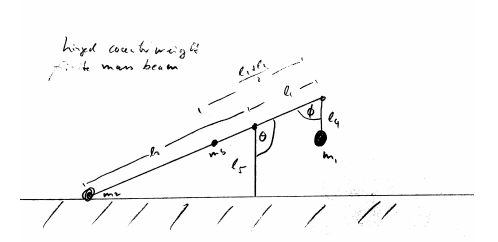
\includegraphics[scale=0.6]{HingedCounterweight.png}
		\caption{Caption}
		%\label{fig:my_label}
	\end{figure}
	\subsection{The Motion before Released}
	For the system, we have the coordinate for mass $m_2$:
	\begin{equation}
	\left\{
	\begin{aligned}
	x&=l_1 \sin\theta + l_4 \sin(\theta + \phi - \pi)\\
	y&=-l_1\cos\theta - l_4 \cos(\theta + \phi - \pi)
	\end{aligned}
	\right.\;,
	\end{equation}
	thus, with $l_1 = l_4$, one has
	\begin{equation}\label{xyy}
	\left\{
	\begin{aligned}
	\dot{x}^2+\dot{y}^2
	&=l_1^2 
	\left[2\dot{\theta}^2+\dot{\phi}^2+2\dot{\theta}\dot{\phi}
	-2\dot{\theta}(\dot{\theta}+\dot{\phi})\cos\phi
	\right]
	\\
	y&= l_1 \left[\cos(\theta + \phi) - \cos\theta\right]
	\end{aligned}
	\right.\;,
	\end{equation}
	therefore, the Lagrangian is
	\begin{equation}
	\begin{aligned}
	L &=
	\frac{m_1 l_1^2}{2}\left[2\dot{\theta}^2+\dot{\phi}^2+2\dot{\theta}\dot{\phi}
	-2\dot{\theta}(\dot{\theta}+\dot{\phi})\cos\phi
	\right]
	+\frac{I\dot{\theta}^2}{2}\\
	&\qquad
	-m_1gl_1\left[\cos(\theta + \phi) - \cos\theta\right]\\
	&\qquad
	-
	g\cos\theta\left(m_2l_2+\frac{m_b(l_2-l_1)}{2}\right)
	\;,
	\end{aligned}
	\end{equation}
	where $I=m_2l_2^2+\frac{m_b}{3}\frac{l_1^3+l_2^3}{l_1+l_2}$ is the moment of inertia of the rod and projectile around the rotational center. 
	
	From the above Lagrangian, we obtained the Euler-Lagrange Equation
	\begin{equation}
	\left\{
	\begin{aligned}
	&I\ddot{\theta} + m_1l_1^2\left[
	(2\ddot{\theta}+\ddot{\phi})(1-\cos\phi)
	+
	(2\dot{\theta}+\dot{\phi})\dot{\phi}\sin\phi
	\right]
	\\
	&\qquad=
	m_1 g l_1[\sin(\theta+\phi)-\sin\theta]
	\\ &\qquad
	+
	\left(m_2l_2+\frac{m_b(l_2-l_1)}{2}\right)g\sin\theta
	\\
	%-------
	&\ddot{\phi} + \ddot{\theta}(1-\cos\phi)  
	=\dot{\theta}^2\sin\phi
	+\frac{g}{l_1}\sin(\theta+\phi)
	\end{aligned}\right.\;.
	\end{equation}
	We numerically solved the equation of motion and the results are showed in Fig.(9).
	\begin{figure}[h]
		\centering
		\includegraphics[scale=0.34
		]{hingedlbk1.eps}
		\caption{The dynamics of $\theta(t),\phi(t)$ for See-saw trebuchet with hinged counterweight. $\theta(t)$ hits zero as $t\approx 0.45\;\mathrm{s}$.}
		\label{range1}
	\end{figure}
	\begin{figure}[h]
		\centering
		\includegraphics[scale=0.32]{hingedlbkRange.eps}
		\caption{The projection distance with respect to launching angle $\theta_R$, with hinged counter weight model.}
		\label{hingedrange}
	\end{figure}
	\begin{figure}[h]
		\centering
		\includegraphics[scale=0.32]{hingedlbkOMG.eps}
		\caption{The dynamics of $-\dot{\theta}(t)$ for See-saw trebuchet with hinged counterweight. It reaches its maximum at $t\approx 0.42\;\mathrm{s}$.}
		\label{hingedOMG}
	\end{figure}
	
	\subsection{Released Angle and its result}
	Suppose the release angle is $\theta_R$ (at $t=t_R$), the projection distance is simply:
	\begin{equation}
	R(\theta_R)
	=
	\frac{v^2(\dot{\theta}_R) \sin 2\theta_R}{g}
	=
	\frac{l_2^2\dot{\theta}_R^2 \sin 2\theta_R}{g}\;.
	\end{equation}
	We obtained the numerical result via this equation, as shown in figure (\ref{hingedrange}). 
	The angular velocity for $\theta$ is also presented in figure (\ref{hingedOMG}). Here we list some results:
	\begin{equation}
	\left\{
	\begin{aligned}
	R_{\mathrm{opt}} &\approx 26.4991 \;\mathrm{m}\;,\qquad
	t_R \approx 0.4125\;\mathrm{s}\\
	\theta_R &\approx 0.4914\;\mathrm{rad}
	\approx 0.1564\pi\;\mathrm{rad}\\
	-\dot{\theta}(t_R) &\approx 14.729\;\mathrm{rad/s}\\ 
	-\dot{\theta}_{\mathrm{max}} &\approx 15.0945\;\mathrm{rad/s}\\ 
	\end{aligned}\right.
	\end{equation}
	Through these result, the maximized range efficiency is
	\begin{equation}
	\epsilon_R(\theta_R)
	=
	\frac{R_{\mathrm{opt}}}{2h m_1  /m_2}
	\approx0.2890
	\end{equation}
	
	One can also find $\dot{\theta}(t_R) = -14.722\;\mathrm{rad/s}$ according to Fig.(\ref{range1},\ref{hingedrange},\ref{hingedOMG}), which yields the energy efficiency at optimal $\theta_R$:
	\begin{equation}
	\epsilon_{E}(\theta_R)=\frac{m_2l_2^2
		\dot{\theta}(t_R)^2}{2m_1g h}
	\approx 0.3476%0.1927\;.
	\end{equation}
	These results are better than those obtained in part(b).
	
	At last, the existence of $m_b$ actually yields an unnecessary rotational energy that \emph{decrease} the efficiency of trebuchet.
	\newline\newpage
	%================
	%================
	\newpage
	\section{The Ultimate Sling model}
	\begin{figure}[h]
		\centering
		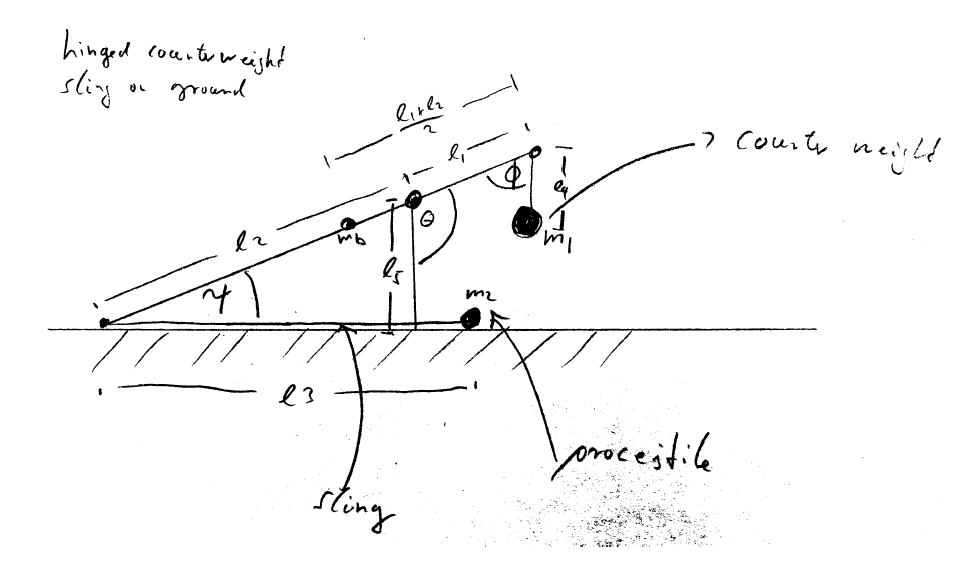
\includegraphics[scale=0.25]{ult.png}
		\caption{The Ultimate Sling model.}
		\label{ultfig}
	\end{figure}
	First, the coordinates for projectile can be expressed in terms of $\theta$ and $\psi$:
	\begin{equation}\label{XYY}
	\left\{
	\begin{aligned}
	X &= -l_2\sin(\pi - \theta) + l_3\cos(\psi+\pi-\theta - \frac{\pi}{2})\\
	& = -l_2\sin\theta + l_3\sin(\theta - \psi)\\
	Y &= -l_2\cos(\pi - \theta)
	- l_3\sin(\psi+\pi-\theta - \frac{\pi}{2})\\
	&=l_2\cos \theta 
	- l_3\cos(\theta - \psi)
	\end{aligned}
	\right.
	\end{equation}
	such that
	\begin{equation}\label{dXdY}
	\begin{aligned}
	\dot{X}^2+ \dot{Y}^2
	&=
	l_2^2\dot{\theta}^2+l_3^2(\dot{\theta}-\dot{\psi})^2
	-
	2l_2l_3\dot{\theta}(\dot{\theta}-\dot{\psi})\cos\psi
	\\
	&=
	(l_2^2+l_3^2-2l_2l_3\cos\psi)\dot{\theta}^2
	+l_3^2\dot{\psi}^2\\
	&\qquad
	-
	2l_3(l_3 - l_2\cos\psi)\dot{\theta}\dot{\psi}
	\end{aligned}
	\end{equation}
	
	Say, the moment of inertia of the rod is $I'=\frac{m_b}{3}\frac{l_1^3+l_2^3}{l_1+l_2}$, together with Eq.(\ref{xyy},\ref{XYY},\ref{dXdY}), our un-constrainted Lagrangian can be written as Eq.(\ref{LLL}):
	%%%%%%%%%
	%------------------
	\begin{widetext}
		\begin{equation}\label{LLL}
		\begin{aligned}
		L
		&=
		\frac{I'\dot{\theta}^2}{2} + \frac{m_1}{2}\left(\dot{x}^2 + \dot{y}^2\right) 
		+ \frac{m_2}{2}\left(\dot{X}^2 + \dot{Y}^2\right)
		%\\&\qquad
		-m_1gy -m_2gY - m_bg\frac{l_2-l_1}{2}\cos\theta\\
		&=
		\frac{I'\dot{\theta}^2}{2} + \frac{m_1 l_1^2}{2}\left[2\dot{\theta}^2+\dot{\phi}^2+2\dot{\theta}\dot{\phi}
		-2\dot{\theta}(\dot{\theta}+\dot{\phi})\cos\phi\right]
		+ \frac{m_2}{2}
		\left[(l_2^2+l_3^2-2l_2l_3\cos\psi)\dot{\theta}^2
		+l_3^2\dot{\psi}^2-
		2l_3(l_3 - l_2\cos\psi)\dot{\theta}\dot{\psi}\right]\\
		&\qquad
		-m_1 gl_1 \left[\cos(\theta + \phi) - \cos\theta\right]
		-m_2 g\left(l_2\cos \theta 
		- l_3\cos(\theta - \psi)\right)
		-m_bg\frac{l_2-l_1}{2}\cos\theta
		\end{aligned}
		\end{equation}
	\end{widetext}
	
	For phase 1, when $\theta \le \theta_L$, one needs to apply Lagrange multipliers when the projectile is sliding on the ground:
	\begin{equation}\label{LnF}
	\begin{aligned}
	L + \lambda f(\psi) &= 
	L + \lambda \left(l_2\cos \theta 
	- l_3\cos(\theta - \psi) + l_2\sin\frac{\pi}{4}\right)
	\;.
	\end{aligned}
	\end{equation}
	In which
	\begin{equation}\label{constr}
	f(\psi)=l_2\cos \theta 
	- l_3\cos(\theta - \psi) + l_2/\sqrt{2} = 0
	\end{equation}
	is the constraint when the projectile is contact with the ground,
	i.e., Eq.(\ref{LnF},\ref{LLL}) yields the Euler-Lagrange equations for $\theta,\psi,\phi$:
	\begin{widetext}
		\begin{equation}\label{eom01}
		\begin{aligned}
		&I'\ddot{\theta}
		+
		m_1l_1^2\left[
		2\ddot{\theta} + \ddot{\phi} - (2\ddot{\theta}+\ddot{\phi})\cos\phi + (2\dot{\theta}+\dot{\phi})\dot{\phi} \sin\phi 
		\right]
		\\&\qquad\qquad
		+
		m_2\left[
		(l_2^2+l_3^2-2l_2l_3\cos\psi)\ddot{\theta} + 2l_2l_3\dot{\psi}\dot{\theta}\sin\psi
		-
		l_3(l_3 - l_2\cos\psi)\ddot{\psi} - l_2l_3\dot{\psi}^2\sin\psi
		\right]
		\\&\qquad
		=
		m_1gl_1\left[\sin(\theta+\phi) - \sin\theta\right] + m_2g\left[l_2\sin\theta - l_3 \sin(\theta - \psi)\right]
		+
		m_bg\frac{l_2 - l_1}{2}\sin\theta
		\\&\qquad\qquad
		+
		\lambda\left[
		l_3\sin(\theta - \psi) - l_2\sin\theta
		\right]\;,
		\end{aligned}
		\end{equation}
		%---------------------------------
		\begin{equation}\label{eom02}
		l_3^2\ddot{\psi} - l_3(l_3 -l_2\cos\psi)\ddot{\theta} 
		=
		l_2 l_3 \dot{\theta}^2 \sin\psi + \left(g-\frac{\lambda}{m_2}\right)l_3 \sin(\theta - \psi) \;,
		\end{equation}
		%--------------------------------
		\begin{equation}\label{eom03}
		\ddot{\phi} + \ddot{\theta}(1-\cos\phi)  
		=\dot{\theta}^2\sin\phi
		+\frac{g}{l_1}\sin(\theta+\phi)\;.
		\end{equation}
	\end{widetext}
	Due to the initial conditions:
	\begin{equation}
	\begin{aligned}
	\theta_0 &= 3\pi/4,\quad
	\phi_0 = \psi_0 = \pi/4\;,\\
	\dot{\theta}_0 &= \dot{\phi}_0 =\dot{\psi}_0 = 0\;,
	%	\\\lambda_0 &= m_2g
	\end{aligned}
	\end{equation}
	We can find the numerical result before the projectile detaches from the ground (as shown in Fig.(\ref{ultdyn},\ref{ultlambda})).
	\begin{figure}[h]
		\centering
		\includegraphics[scale=0.34]{ultlbk1.eps}
		\caption{The evolution of $\theta(t),\;\phi(t),\;\psi(t)$. The verticle dash line shows the moment when the projectile detaches from the ground.}
		\label{ultdyn}
	\end{figure}
	\begin{figure}[h]
		\centering
		\includegraphics[scale=0.34]{lambdalbk1.eps}
		\caption{The evolution of supporting force $\lambda(t)$. It hits zero at $t_L \approx 0.1691\;\mathrm{s}$.}
		\label{ultlambda}
	\end{figure}
	\begin{figure}[h]
		\centering
		\includegraphics[scale=0.34]{ulttot.eps}
		\caption{The total evolution of $\theta(t),\phi(t),\psi(t)$ before and after the projectile detaches the ground ($t = t_L$, vertical dashed line). (One can verify the energy conservation through this.)} 
		\label{ultddyn}
	\end{figure}
	
	We find the data at detaching moment ($t=t_L\approx 0.1691\;\mathrm{s}$) is:
	\begin{equation}\label{dataL}
	\left\{
	\begin{aligned}
	\theta_L &\approx 1.9900\;\mathrm{rad} \approx 0.633\pi\;\mathrm{rad}
	\\
	\phi_L &\approx 0.9511\;\mathrm{rad}\approx 0.3027\pi\;\mathrm{rad}
	\\
	\psi_L &\approx 0.7876\;\mathrm{rad} \approx 0.2507\pi\;\mathrm{rad}
	\\
	\dot{\theta}_L &\approx -4.0758\;\mathrm{rad/s}\\
	\dot{\phi}_L &\approx 2.5360\;\mathrm{rad/s}\\
	\dot{\psi}_L &\approx 0.7129\;\mathrm{rad/s}\\
	\end{aligned}\right.\;.
	\end{equation}
	
	Utilizing the conditions from (\ref{dataL}), one can solve equations of motion (\ref{eom01},\ref{eom02},\ref{eom03}) numerically with $\lambda \equiv 0$, since the ground no longer acting on the projectile. One obtains the result of the total evolution before release in Fig.(\ref{ultddyn}).
	
	
	In the end, the projection range can be calculated through
	\begin{equation}
	R = \dot{X}\cdot \Delta t =  \frac{2 \dot{X}\dot{Y}}{g}\;,
	\end{equation}
	where the size of trebuchet has been ignore.
	The numerical relation of range $R$ versus release angle $\theta_R$ is plotted in Fig.(\ref{ultrange}), which obviously shows the optimized range is largely extended:
	\begin{equation}
	R_{\mathrm{opt}}\approx 74.1996\;\mathrm{m}\;.
	\end{equation}
	\begin{figure}[h]
		\centering
		\includegraphics[scale=0.33]{ultRange.eps}
		\caption{The relations between release angle $\theta_R$ and the projection range $R(\theta_R)$, with the optimized range $R_{\mathrm{opt}}\approx 74.1996\;\mathrm{m}$. Only in a particular range of $\theta_R$ one has positive projection range.}
		\label{ultrange}
	\end{figure}
	When this optimized range is reached, the trebuchet has such launching configuration :
	\begin{equation}
	\left\{
	\begin{aligned}
	\theta_R &\approx 0.1800\;\mathrm{rad} \approx 0.0573\pi\;\mathrm{rad}\\
	\phi_R &\approx 3.5540\;\mathrm{rad} \approx 1.1313\pi\;\mathrm{rad}\\
	\psi_R &\approx 2.5033\;\mathrm{rad} \approx 0.7968\pi\;\mathrm{rad}\\
	\dot{\theta}_R &\approx -1.9654\;\mathrm{rad/s}\\
	\dot{\phi}_R &\approx 2.0805\;\mathrm{rad/s}\\
	\dot{\psi}_R &\approx 23.0797\;\mathrm{rad/s}\\
	y_R &=-0.5440\;\mathrm{m}\\
	v_R^2 &= \dot{X}_R^2 + \dot{Y}_R^2 \approx 727.6964\;\mathrm{m^2/s^2}
	\end{aligned}
	\right.
	\end{equation}
	which yields the falling distance of $m_1$ is $h = y(0) - y_R \approx 0.4562\;\mathrm{m}$, then the efficiencies are
	\begin{equation}
	\begin{aligned}
	\epsilon_R &=\frac{\frac{v_R^2}{g}\sin(2\arctan{\frac{\dot{Y}_R}{\dot{X}_R}})}{2\frac{m_1}{m_2}h}\approx 0.8133\\
	\epsilon_E &=\frac{m_2v_R^2}{2m_1gh}\approx 0.8139
	\end{aligned}\;.
	\end{equation}
	

\section{How to Construct a more Efficient Trebuchet}
From the calculations above, it is obvious that we have two ways to construct a more efficient trebuchet. The first one is to decrease the work done to other part of the trebuchet except the projector, the second on is to let the projectile angle closer to $\pi/4$.
\subsection{Decrease Wastage of Energy}
We have two ways to decrease the wastage of energy.
\begin{enumerate}
    \item Decrease the mass of the rod. When we decrease the mass of the rod, we will spend less energy on rotate the rod. Therefore, the energy on the projectile will increase.
    \item Decrease the velocity of the rod and hanging weight at the projected moment.
    \item Increase the hinges number properly could increase the efficiency of energy.
\end{enumerate}
\subsection{Make the Projected Angle Closer to $\pi/4$}
In order to make the projected angle closer to $\pi/4$, we can adjust the ratio between $l_3$ and $l_4$. With a proper ratio, we may have the maximum initial velocity of the projector with a projected angle of $\pi/4$, which will give us the largest range. However, since the projectile is accelerating, the best angle that optimizes the range is usually deviating from $\pi/4$.

\end{document}
%
% ****** End of file apssamp.tex ******